\documentclass{article}

\usepackage{graphicx}
\usepackage{pgffor}
\usepackage{listings}
\usepackage{color}

\usepackage{datatool}

\definecolor{dkgreen}{rgb}{0,0.6,0}
\definecolor{gray}{rgb}{0.5,0.5,0.5}
\definecolor{mauve}{rgb}{0.58,0,0.82}

%% footnote size proved perfect here for getting the code to appear as 80 chars
%% wide like standard

\lstset{frame=tb,
  language=Python,
  aboveskip=3mm,
  belowskip=3mm,
  showstringspaces=true,
  columns=flexible,
  basicstyle={\footnotesize\ttfamily},
  numbers=none,
  numberstyle=\tiny\color{gray},
  keywordstyle=\color{blue},
  commentstyle=\color{dkgreen},
  stringstyle=\color{mauve},
  breaklines=true,
  breakatwhitespace=false,
  tabsize=3
}


\begin{document}



\newpage
   \vspace*{\stretch{1.0}}
   \begin{center}
      \Large\textbf{Earth 436B Thesis}\\
      \large\textit{John Lawson}
   \end{center}
   \vspace*{\stretch{2.0}}

\newpage


\tableofcontents
\newpage




\DTLloaddb{result}{data/bothNonZero_withinSeventyFivePercent_intervals.csv}
\newcommand{\result}[1]{%
    \dtlgetrowforvalue{result}{\dtlcolumnindex{result}{id}}{#1}%
    % read variables into commands
\dtlgetentryfromcurrentrow{\id}{1}
\dtlgetentryfromcurrentrow{\name}{2}
\dtlgetentryfromcurrentrow{\startValue}{3}
\dtlgetentryfromcurrentrow{\endValue}{4}

% use commands in text
\text{\startValue} to \text{\endValue} cm/century

%
}


\section{Abstract}

The ground surface underlying the Laurentian Great Lakes is currently undergoing vertical adjustment
 after being depressed by the weight of an ice sheet formed in the most recent glacial period during the Wisconsonian.
 The rate of glacial isostatic adjustment (GIA) varies by location, and strongly influences the flow of water
 in the Laurentian Great Lakes (LGL) as the inclination of the ground surface changes. Previous attempts to 
 estimate the rate of GIA between sites used geologically recent water gauge data from the
 past 200 years in order to measure the rate of GIA. In contrast, by
 inferring GIA from measurements of the water level in the geological record over the past 5000 years,
 a more accurate estimate of the long term process of GIA can be obtained. These measurements are
 made by measuring the elevation of a subsurface sedimentary contact relating to
 past lake levels,which are then age dated with optically stimulated luminescence
 (OSL) to provide an age for sediments. Elevation and age data are then compiled
 to create site paleohydrographs for each location around the lake basin.\\
 
 The focus of this paper is to analyze the data compiled by Johnston et al, 2014
 which measured past elevation of shorelines by interpreting water levels recorded
 in the sediment record. Each site paleohydrograph
 is now extended between points where the data was measured directly, then subtracted
 from one data point to a modelled elevation in order to create a
 plot of relative elevation over time. Once this is done, the rate of change per unit
 time is obtained from a linear regression, representing an estimate of the value
 of GIA between each pair of sites. This process is repeated for
 all possible combinations of the four sites used, 
 Grand Traverse Bay (GTB), Au Train Bay (ATB), Batchawana Bay (BATB), and Tahquamenon Bay (TAHB).\\
 
 
 
 The results of this process were in strong agreement at the 95 \% confidence level for GIA rates obtained from
 forward and reverse regressions for the combination of ATB-BATB (23.5 to 31 cm/century) and
 BATB-TAHB (11 to 17 cm/century). Agreement was also seen at the 95 \% confidence level for GTB-TAHB (anywhere from -3 to 8.5 cm/century),
 ATB-GTB (9 to 13 cm/century) and ATB-TAHB (19.5 to 29 cm/century).

\newpage

\section{Introduction}
 The Earths crust rests on top of the mantle, its elevation rising and falling
 with the amount of mass weighing on it. During glacial periods, a significant portion
 of the water on earth is transferred in form from water in the oceans to glacial ice sheets,
 weighing down the continental crust and causing the mantle to dynamically adjust
 with it. This causes the crust to ride relatively lower in elevation,
 a change which reverses when the weight is removed as the ice sheets melt.
 This vertical motion of the crust while attempting to returning to its previous position is known
 as glacial isostatic adjustment (GIA) (Scott et al, 2010).\\
 
 The process of GIA has implications for the routes that the flow
 of water on the Earths surface takes; the "tilting" of the surface caused by 
 uneven rates of GIA in different locations (the thickness and residence time of
 the ice sheet impacts how much the crust subsides and how rapidly it rebounds) 
 may open or close drainage outlets from basins, possibly
 causing some rivers and lake outlets to go dry, while opening new ones as the
 'tilt' of the lake basin changes.
 Additionally, the change in "tilt" has potential to change shorelines of existing
 basins, which has implications for land usage and long term engineering
 projections for structures such as locks and dams, where the usage lifetime of
 the structure may extend over decades or centuries.\\

\newpage
\section{Previous Work} 
Mainville \& Craymer (2005) used water gauge data collected around the LGL over the past 150 years to
 create monthly means of water level. Differences in these values between sites
 were then plotted against time to calculate a rate of elevation change between
 sites over time (This value is interpreted to represent the impact of the GIA
 process on the crust underlying the LGL, even though the actual process extends
 over a much longer timescale than that of the data collection). Combinations of sites were shown to produce
 inconsistent results, so a second method using a least squares adjustment process was used,
 removing some monthly mean outliers which plotted at or beyond some arbitrary residual distance away 
 from the linear regression line in the vertical (elevation) axis. 
 This process was repeated with each new linear regression on the remaining data
 points until none remained "too far away" from
 the final regression line. A third, and ultimately optimal method for calculating
 GIA was developed by
 Mainville \& Craymer in their 2005 paper, this time computing velocity at a given
 month from the difference between a
 the monthly water level mean and an reference water level for the epoch that the 
 month is found in (this 
 reference level being adjusted for epoch
 and site biases). This elevation difference is then divided by the time difference
 between the start of the epoch and the month that was measured, calculating a rate
 of GIA for the month measured. Their findings with this method showed a general agreement with the post glacial
 ICE-3G global model of GIA at that time, while the ICE-4G model developed by Peltier
 was shown to underestimate the relative difference in vertical movement across
 the span of the Great Lakes (Mainville \& Craymer, 2005).\\ \\
Johnston et al. (2012) attempted to provide a value for GIA in the LGL with
 better accuracy than previous estimates calculated using water
 gauge data.
 
In order to accomplish this, the data used to measure the process of
 GIA needed to extend over a much longer timescale. In this method, water
 levels were inferred from the elevation of relict shorelines in beach ridge
 strandplains from the late Holocene sediment record surrounding Lake Superior.
 Ages for each elevation were inferred from age dating samples from these beach
 deposits (known as strandplain sequences) using
 optically stimulated luminescence (OSL) age dating. Johnston et al (2012) differed from
 Mainville \& Craymer (2005), in that data collected for the 2012 paper using OSL
 age dating did not have
 elevations sampled at the same points in time for calculation of relative
 rates. As a result, Johnston et al (2012) the elevation vs time data was modelled with a linear
 regression for each site, the difference in slopes of each regression representing the GIA rate
 between sites. Individual regressions were further created per site
 for a series of four ranges of time related to lake level phases, namely the Nipissing,
 Algoma, Sault, and Sub-Sault (Johnston et al, 2012). The results reported from this process
 are summarized in Figure \ref{fig:jj2012Grid}. \\
 
 \begin{figure}[t]
	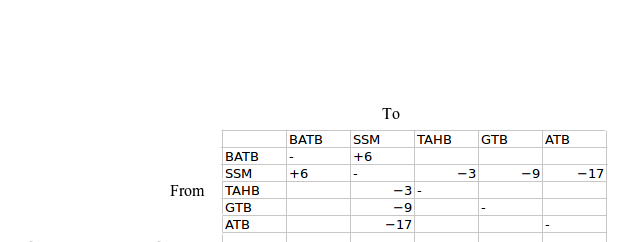
\includegraphics[width=0.9\linewidth]{jjGrid.png}
	\caption{GIA values reported by Johnston et al 2012. All values are in cm/century.}
	\label{fig:jj2012Grid}
 \end{figure}
 % need to ask JJ about JJ 2012, bottom of page 3, divergence of intercepts
 

 
 In order to project the future impact of this process on the Great Lakes Basin,
 an estimate of the historical rate of GIA is needed. This estimate is obtained by
 comparing the elevation of the water mark at two different locations around a basin, and
 observing how this difference changes over time. The elevation of the water can be inferred
 by a variety of indicators in the sediment record, in this case, beach deposits known
 as strandplain sequences are used, their ages determined by optically stimulated
 luminescence (OSL) dating. This raw data is presented in Figure \ref{fig:rawData}.\\
\begin{figure}[h]
	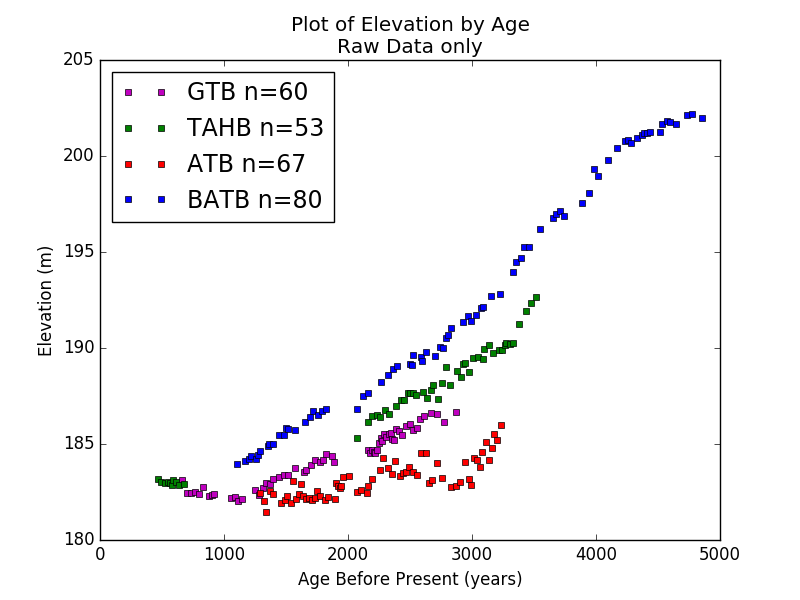
\includegraphics[width=1.1\linewidth]{data/theDataRaw.png}
	\caption{Current day elevation of relict shorelines with respect to time before present over the last 5000 years. Strandplain sites Au Train Bay, Michigan (ATB), Batchawana Bay, Ontario (BATB), Tahquamenon Bay, Michigan (TAHB), and Grand Traverse Bay, Michigan (GTB) surrounding Lake Superior are plotted individually. Data from Johnston et al, (2012)}
	\label{fig:rawData}
\end{figure} 
%\begin{figure}[h]
	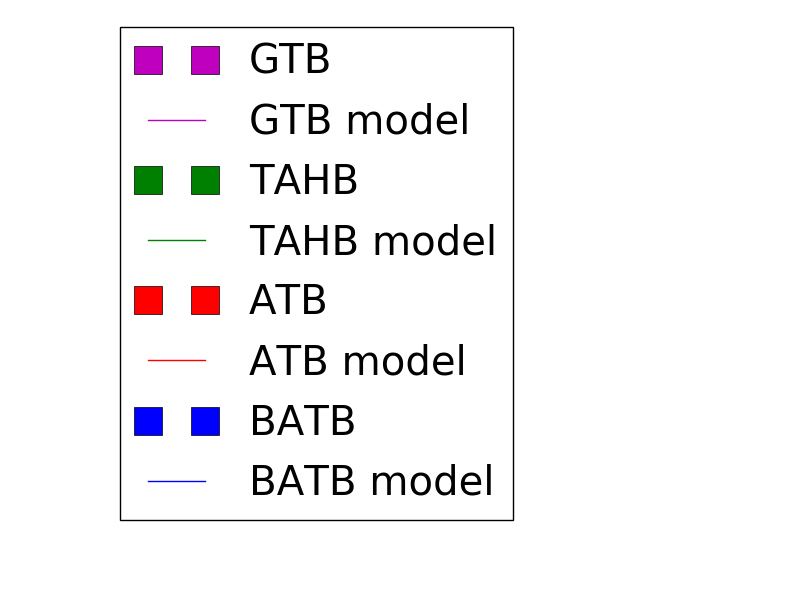
\includegraphics[width=0.40\textwidth]{data/legendary.png}
	%\makebox[\textwidth]{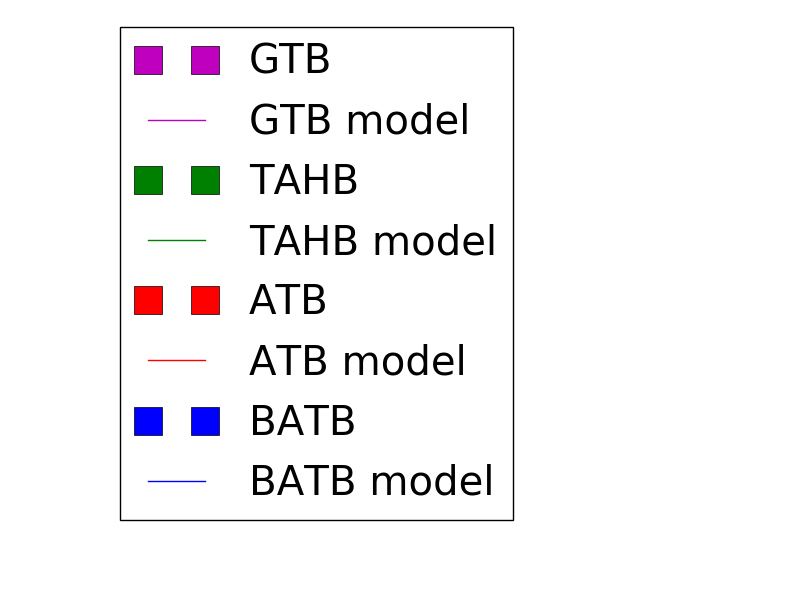
\includegraphics[width=\paperwidth]{data/legendary.png}}
	%\caption{Site Legend}
	%\label{fig:rdmLegend}
\end{figure}



\newpage 
 
 The data was sampled from four separate locations around Lake Superior, namely
 Au Train Bay, Michigan (known in this paper as ATB), Grand Traverse Bay,
 Michigan (known as GTB), Batchawana Bay, Ontario (known as BATB), and 
 Tahquamenon Bay, Michigan (TAHB).\\
 \begin{figure}[h]
	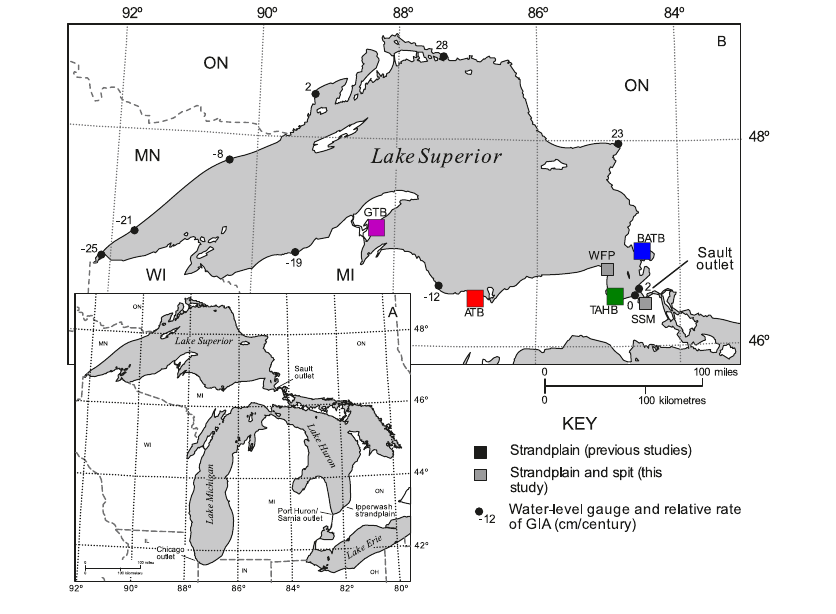
\includegraphics[width=0.8\linewidth]{johnstonLaurentianMapWithSites.png}
	\caption{Geographic Map of Lake Superior \& surrounding regions. Note that
	 the colour of each site marker will remain constant throughout the rest of
	 this paper for convenience. Reproduced from Johnston et al, 2014}
	\label{fig:johnstonLaurentianMapWithSites}
 \end{figure}

 These datasets were previously created by
 Johnston et al, 2014, but were analyzed using a different method.
 From observing the graph, it can be seen that all four datasets follow somewhat
 linear trends, increasing in elevation as the time before present increases.
 This is because the crust underlying the Great Lakes has been rebounding upwards
 over the time period in question, implying that areas that were at the
 elevation of the water surface in the past have been shifted up in elevation
 above the current water surface elevation. The rate of this upward trend varies
 by site, generally increasing for sites closest to the north and east extremes.
 (this is due to the rate of rebound increasing with closeness to the center of
 the Laurentide Ice Sheet, roughly near current day James Bay in Northern Ontario).\\
 Between the four sites, the most common feature is good data coverage between
 1000 and 3500 years before present, with a common gap in coverage around 2000
 years before present. This was due to conditions which worked against the
 formation of strandplain sequences during the Algoma lake level fluctuation
 (Johnston et al, 2014), thus causing most of our datasets to have interrupted
 records of lake level elevation at this time. While some of the datasets have
 coverage extending far beyond this range, the only dataset which does not follow
 this pattern of data coverage is TAHB, which will be discussed later in this section.\\ 
 In order to measure a relative rate of GIA between sites, the rate at which these
 trends diverge must be measured. In the previous work done on this dataset, this
 was accomplished by representing the trend of increasing elevation with age as
 a straight line using a linear regression (Johnston et al, 2014). This was an
 effective first approximation, but failed to take into account that large gaps
 exist the ranges of time before present where no data is available for some
 sites. For example, the TAHB dataset has a large gap between 600 and 2100 years
 before present in which no data is available. A linear regression of this dataset
 would imply a similar rate of change connecting these two disconnected ranges,
 during which there is no actual evidence that the sites actual elevation was
 anywhere near the linear regression line. which it is represented by in
 calculations for producing a GIA rate.\\
 In order to produce an estimate of GIA which better reflects the inconsistent
 coverage of the data over time, a better strategy would be to simply subtract
 the differences in elevation between sites and plot these differences with
 respect to time. Unfortunately however, none of the datasets have elevations
 sampled at the same times, an estimate of elevation being needed for times where
 one dataset
 has a data point present, but the other does not. In this paper, this estimate 
 (the modelled elevation) is created by using linear interpolation between datapoints,
 represented as a solid line between points as seen in Figure \ref{fig:rawDataWithModel}.\\
\begin{figure}[h]
	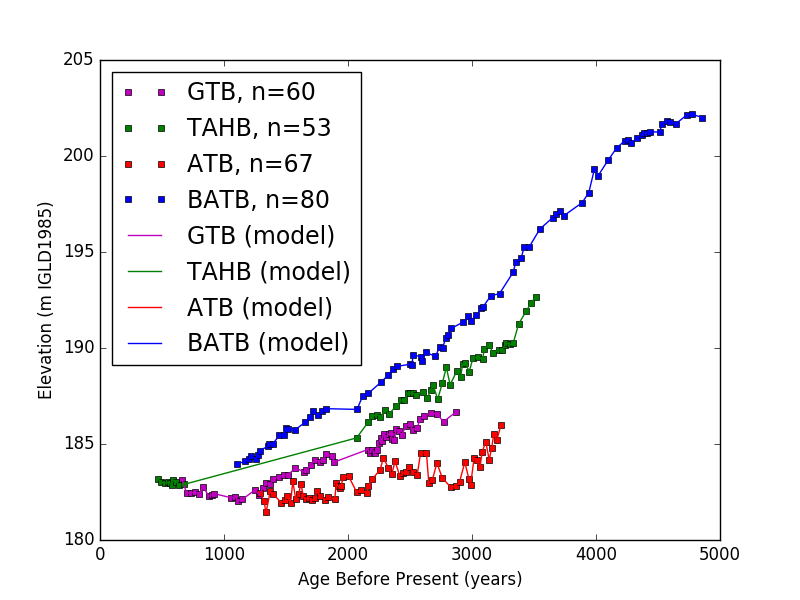
\includegraphics[width=\linewidth]{data/theData.png}
	\caption{Water surface elevation with respect to time before present, modelled}
	\label{fig:rawDataWithModel}
\end{figure}
\newpage
%\begin{figure}[h]
	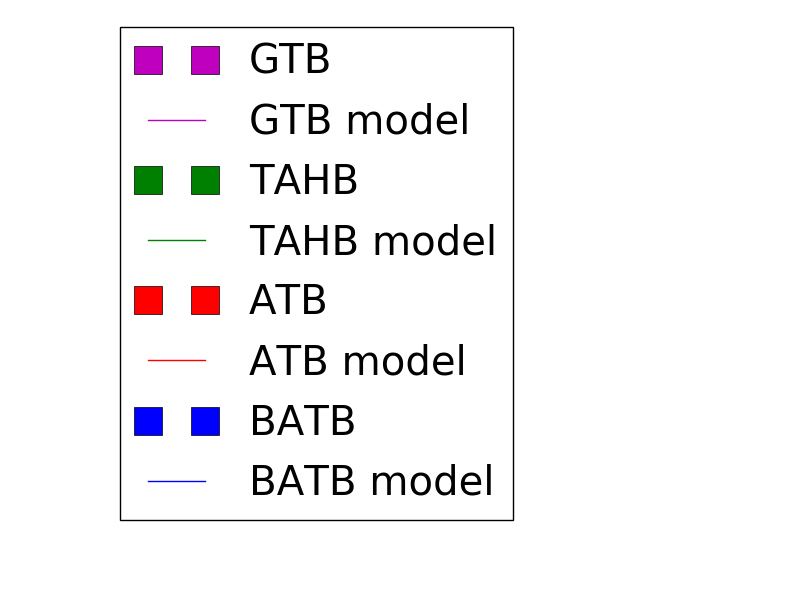
\includegraphics[width=0.40\textwidth]{data/legendary.png}
	%\makebox[\textwidth]{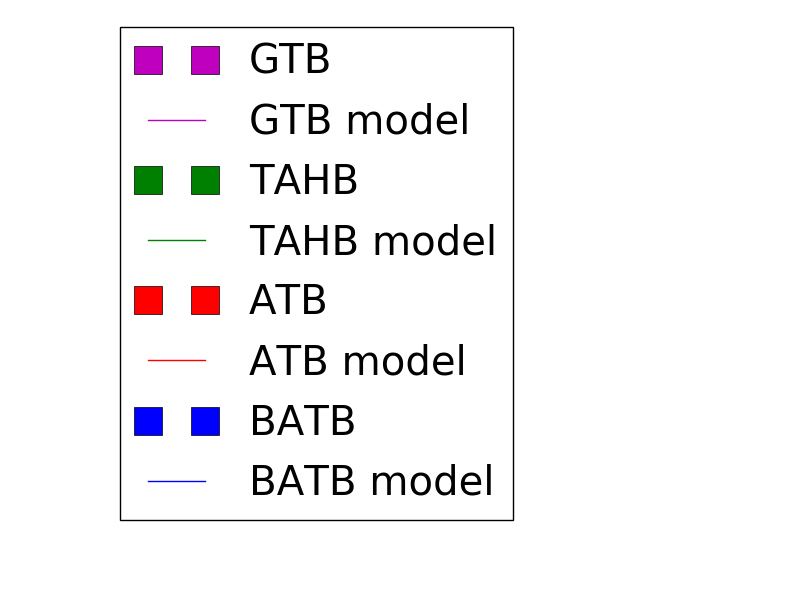
\includegraphics[width=\paperwidth]{data/legendary.png}}
	%\caption{Site Legend}
	%\label{fig:rdmLegend}
\end{figure}


 \subsection{Methods}
 Once this estimate of elevation for times between sampled datapoints at a site
 is created, the difference in gia between sites can be created by subtracting
 the elevation of a measured data point from the modelled elevation of another
 dataset at that point in time, this difference is the dashed line shown in
 Figure \ref{fig:rawDataWithModelZoomed}:
 \begin{figure}[h]
	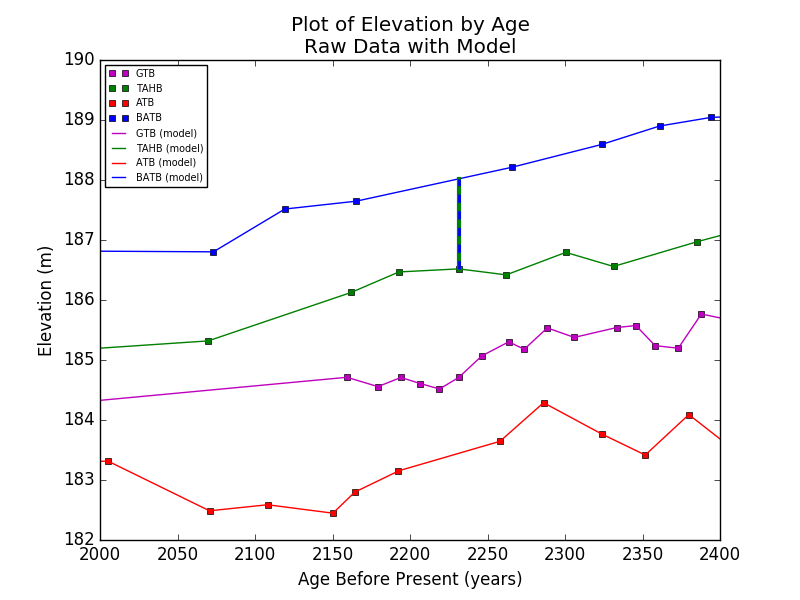
\includegraphics[width=1.1\linewidth]{data/theDataZoomed.png}
	\caption{Example GIA comparison from a data point to a linear interpolation
	model, represented by an alternating dashed line}
	\label{fig:rawDataWithModelZoomed}
 \end{figure}
 To avoid making comparisons between data in one dataset and a model for another
 in areas where the model stretched over long distances between measured data
 (such as the 1500 year gap in TAHB), the data was grouped into a series of bins
 starting at 450 years before present with width of 200 years (ie the error bounds
 on the age values reported in the original data). If any bin had no data
 available for one site or the other in a comparison, none of the datapoints in
 that bin range were used to make comparisons, thus ensuring that areas like the
 gap in TAHB were avoided when making comparisons. In addition, a second rule
 that the counts for the bins needed to be within 75\% of one another was used,
 which cleared up a few areas where the datasets for both bins compared poorly,
 but produced valid comparison windows (see the small zone of GTB-TAHB overlap
 at \~ 600 years before present).

\newpage


\subsection{GIA Calculation Results}



 Listed in this section are the results of each of the possible combinations of sites.
 Since 4 sites were used, a total of 6 distinct combinations of sites were studied.
 For each combination of sites (for example ATB \& BATB) two sets of comparisons
 were made. In the case of ATB \& BATB, the measured elevations from ATB would be
 subtracted to the linear interpolation model of BATB, then the measured elevations
 from BATB would be subtracted to the linear interpolation model of ATB, thus
 creating a pair of plots of elevation differences vs time. Once compiled, a linear
 regression was applied to this 


\subsubsection{ATB-BATB}

\begin{figure}[H]
	\makebox[\textwidth]{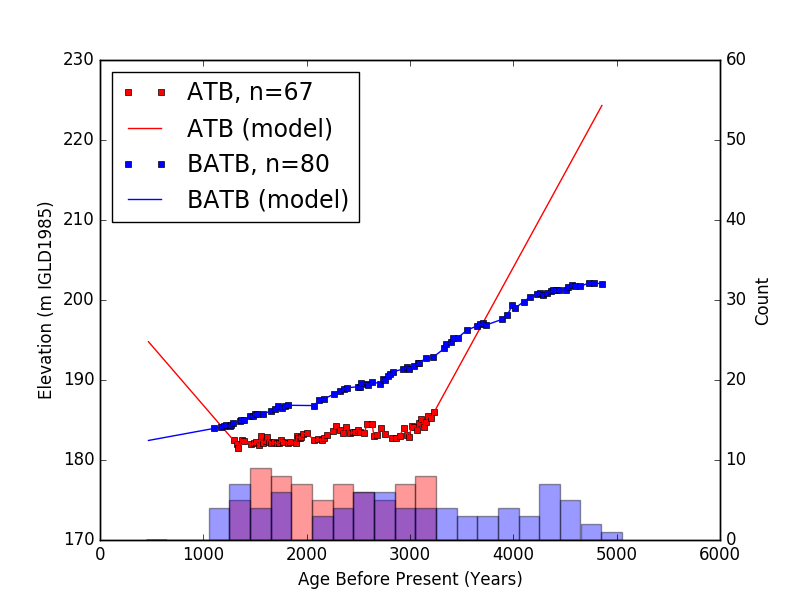
\includegraphics[width=0.72\paperwidth]{data/ATB-BATB_DataAndModel.png}}
	\caption{Measured and modelled elevation data plotted against age for sites ATB \& BATB. Data grouped into bins with widths of 200 years starting at 450 years before present. Bin Counts shown as a histogram at bottom of graph.}
	\label{fig:data_ATBxBATB}
\end{figure}
The data available for sites ATB and BATB shows two of the most common trends in
 the data used in this paper; Data is available for both sites from
 approximately 1000 to 3300 years before present,
 with a gap in the record at around 2000 years before present (caused by a low
 water level period preferentially not forming beach deposits during this time)
 (Johnston et al, 2014). With the data divided up into bins of 200 years width
 starting at 1050 years before present, the data from every bin between 1250 and 3250 was used
 in calculating a rate of GIA, save for the gap from 1850-2050 years before
 present caused by the Algoma low water level (where comparisons between data in the ATB dataset would be
 subtracting against a modelled value for BATB that is unreliable given
 the distance to the nearest datapoint in BATB). The regressions derived from this pair of data sets,
 seen in Figures \ref{fig:gias_ATBxBATB} \& \ref{fig:gias_BATBxATB}, are well
 constrained, and produce a moderately well constrained value on relative GIA
 between ATB and BATB of 24.7 - 31.0 cm/century. In order to produce this range, a
 regression was done on both comparisons, the results of which can be seen in
 Figure \ref{fig:ATBxBATB_regression}. The absolute rate of GIA was determined from the
 absolute value of the slopes of each regression, reported here as a 95\% confidence interval
 in cm/century. Once these 95\% intervals were created, a final value was created
 from the range where both confidence intervals overlapped. (for example, with this
 site the two ranges are -24.71 to -31.01 and 23.51 to 31.45 cm/century. Converting
 to absolute value, the overlap between (24.71,31.01) \& (23.51,31.45) is the range
 (24.71,31.01) ). A complete plot of the confidence intervals
 for the slopes obtained from every linear regression done in this paper can be seen in Figure \ref{fig:intervalsGIA}. \\
24.708,31.013

\begin{figure}[H]
	\begin{flushleft}
	\csvautotabular[respect all]{data/ATB-BATB_regressionTable_bothNonZero_withinSeventyFivePercent.csv}
	\end{flushleft}
	\caption{ATB-BATB Regression output parameters}
	\label{fig:ATBxBATB_regression}
\end{figure}

\newpage

\begin{figure}[H]
	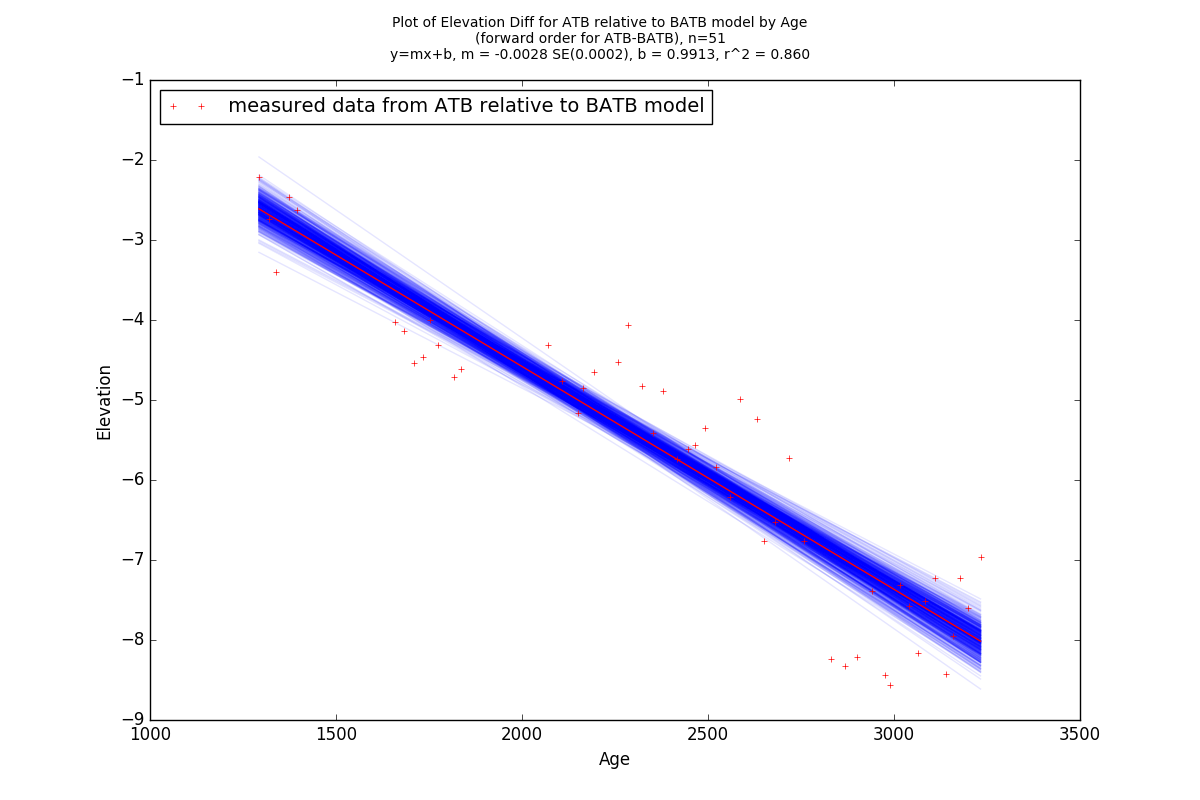
\includegraphics[width=1.7\linewidth, angle=270 ]{data/bothNonZero/withinSeventyFivePercent/gias/theGIA_ATB_relative_to_BATB.png}
	\caption{Differences in elevation measured from the ATB data to the BATB model. 95p Bootstrap of the main regression rendered in blue around the estimator version of the regression (rendered as a solid red line).}
	\label{fig:gias_ATBxBATB}
\end{figure}


\begin{figure}[H]
	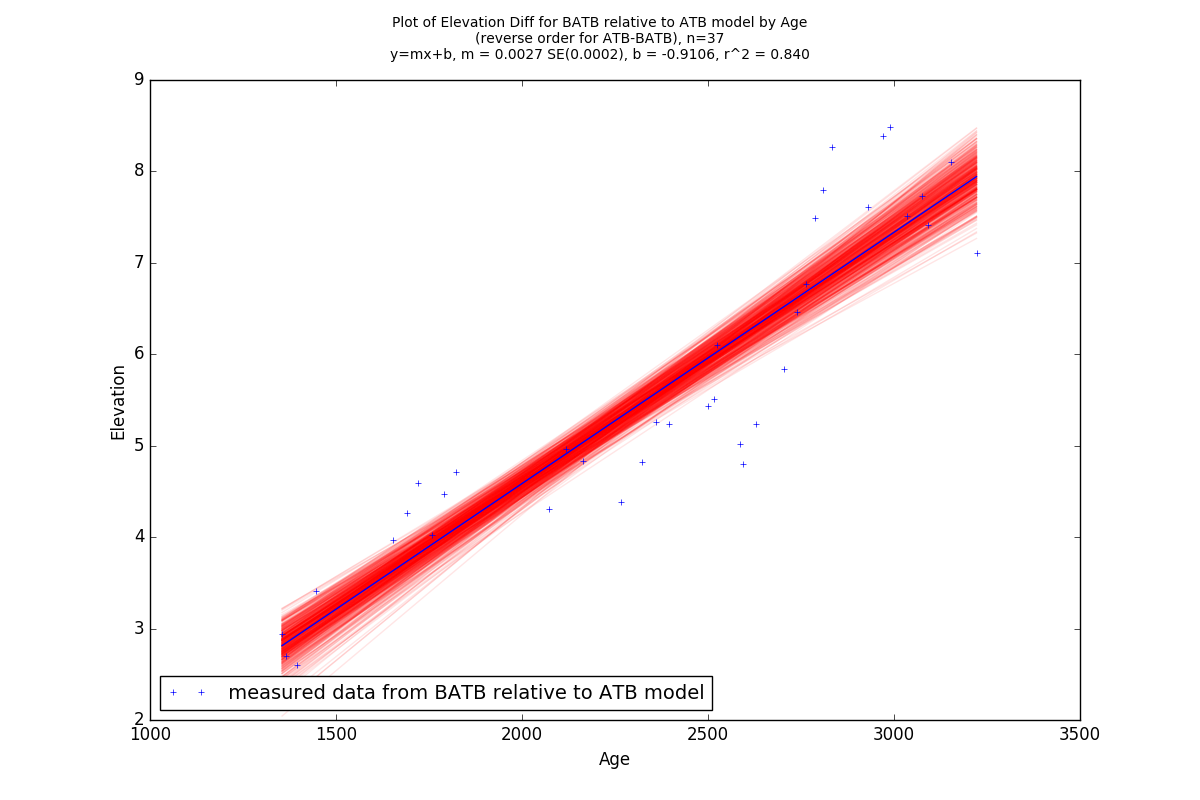
\includegraphics[width=1.7\linewidth, angle=270 ]{data/bothNonZero/withinSeventyFivePercent/gias/theGIA_BATB_relative_to_ATB.png}
	\caption{Differences in elevation measured from the BATB data to the ATB model. 95p Bootstrap of the main regression rendered in red around the estimator version of the regression (rendered as a solid blue line).}
	\label{fig:gias_BATBxATB}
\end{figure}
\newpage
% this desperately needs to be done as a loop













\subsubsection{TAHB-BATB}

\begin{figure}[H]
	\makebox[\textwidth]{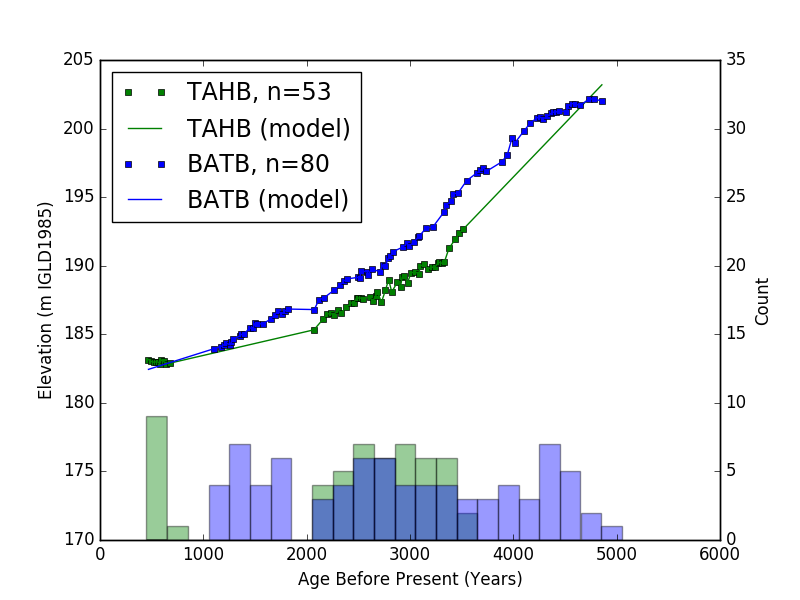
\includegraphics[width=0.72\paperwidth]{data/TAHB-BATB_DataAndModel.png}}
	\caption{Measured and modelled elevation data plotted against age for sites TAHB \& BATB. Data grouped into bins with widths of 200 years starting at 450 years before present. Bin Counts shown as a histogram at bottom of graph.}	
	\label{fig:data_TAHBxBATB}
\end{figure}

The data plot for the site combination of TAHB and BATB shows a common issue
with comparing datasets, as the data with ages more recent than the 2000 year before
present gap is unusable. This is because the regions where data is available for
one dataset are empty of datapoints for the other, making the modelled prediction
of the other dataset unreliable. As a result, a filter is applied to the
data to prevent this, grouping data points into bins 200 years wide starting at 450 years before present, and
ignoring the data points from bins in which either data set had no datapoints,
as well as any which had bin counts differing by more than 75\% for that bin.
As a result, only the data from 2050 to 3650 years before present were used in
creating the GIA comparisons between TAHB and BATB.\\
The linear regressions produced from this pair of datasets are shown in Figures 
\ref{fig:gias_TAHBxBATB} \& \ref{fig:gias_BATBxTAHB}, with the parameters for each
regression listed in Figure \ref{fig:TAHBxBATB_regression}. Merging the two ranges
reported under the "Slope C.I. (95p)" column in Figure \ref{fig:TAHBxBATB_regression},
a value for relative GIA of between 11.9-16.8 cm/century is seen. \\


\begin{figure}[H]
	\begin{flushleft}
	\csvautotabular[respect all]{data/TAHB-BATB_regressionTable_bothNonZero_withinSeventyFivePercent.csv}
	\end{flushleft}
	\caption{TAHB-BATB Regression output parameters}
	\label{fig:TAHBxBATB_regression}
\end{figure}


\newpage

\begin{figure}[H]
	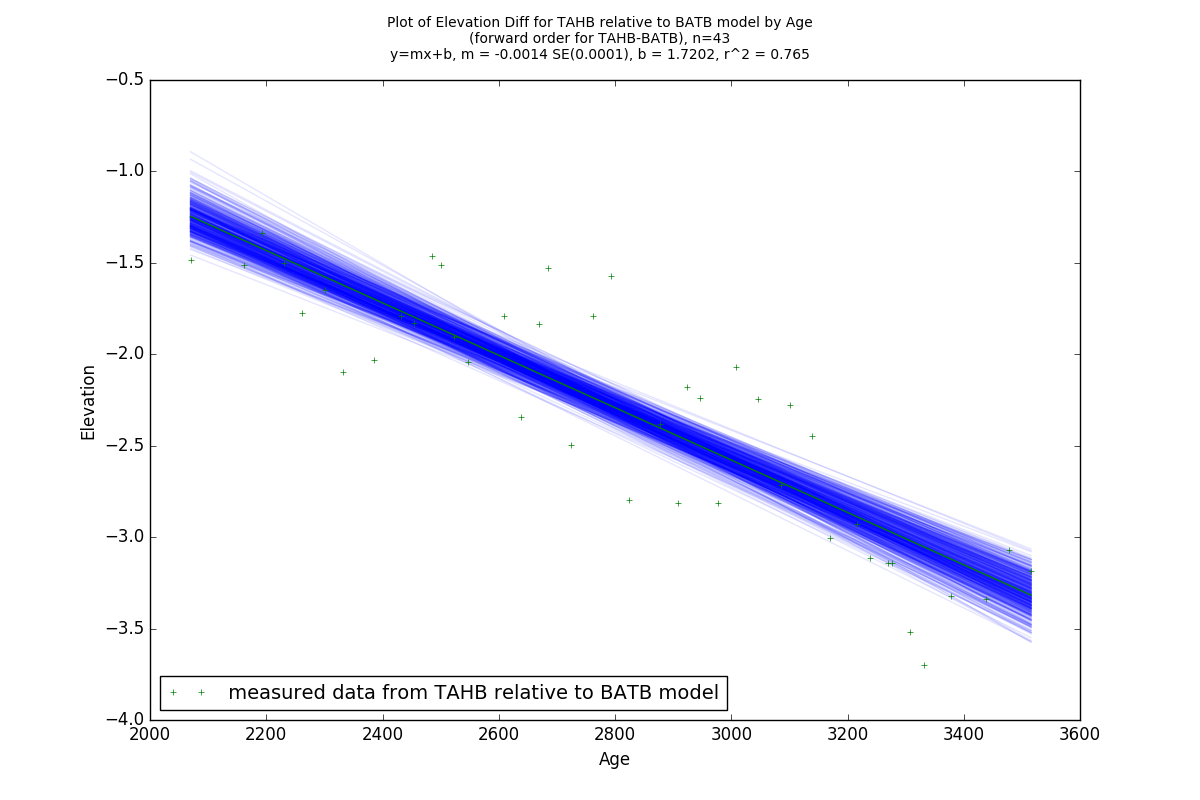
\includegraphics[width=1.7\linewidth, angle=270 ]{data/bothNonZero/withinSeventyFivePercent/gias/theGIA_TAHB_relative_to_BATB.png}
	\caption{Differences in elevation measured from the TAHB data to the BATB model. 95p Bootstrap of the main regression rendered in blue around the estimator version of the regression (rendered as a solid green line).}
	\label{fig:gias_TAHBxBATB}
\end{figure}
\newpage


\begin{figure}[H]
	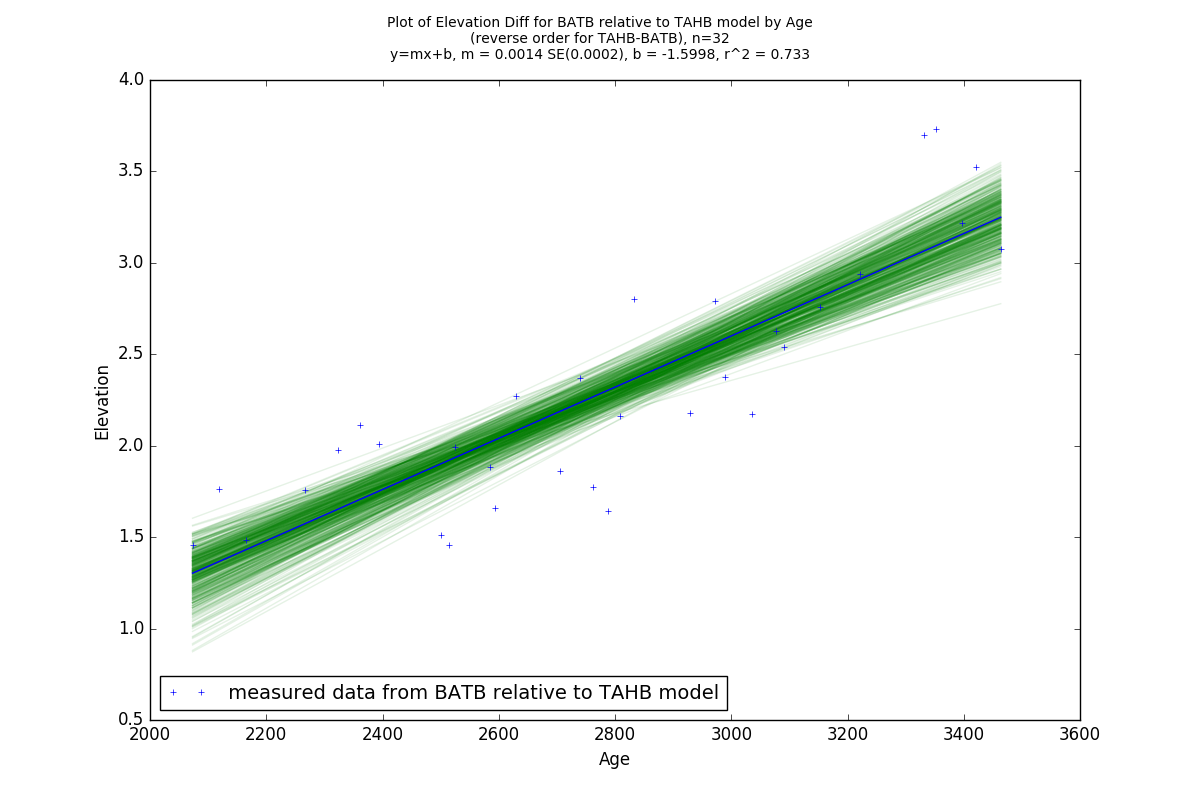
\includegraphics[width=1.7\linewidth, angle=270 ]{data/bothNonZero/withinSeventyFivePercent/gias/theGIA_BATB_relative_to_TAHB.png}
	\caption{Differences in elevation measured from the BATB data to the TAHB model. 95p Bootstrap of the main regression rendered in green around the estimator version of the regression (rendered as a solid blue line).}
	\label{fig:gias_BATBxTAHB}
\end{figure}
\newpage






\subsubsection{TAHB-ATB}

\begin{figure}[H]
	\makebox[\textwidth]{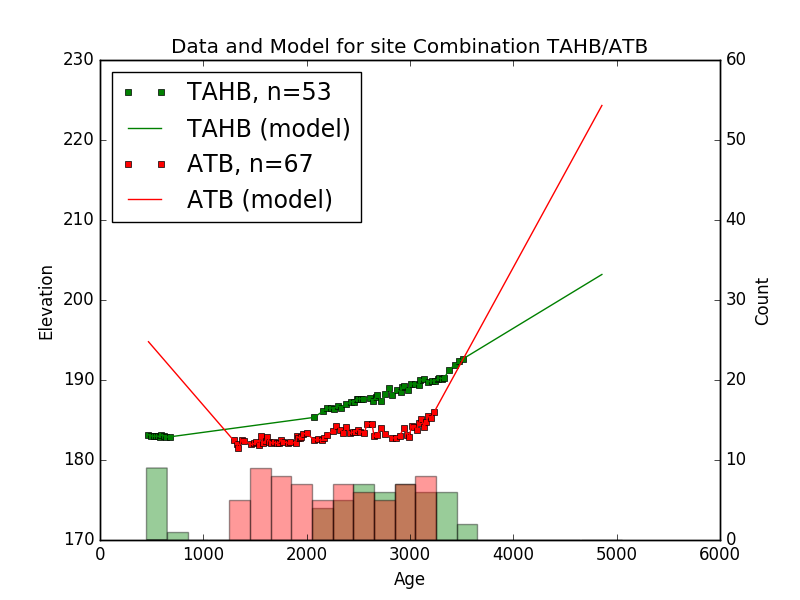
\includegraphics[width=0.72\paperwidth]{data/TAHB-ATB_DataAndModel.png}}
	\caption{Measured and modelled elevation data plotted against age for sites TAHB \& ATB. Data grouped into bins with widths of 200 years starting at 450 years before present. Bin Counts shown as a histogram at bottom of graph.}	
	\label{fig:data_TAHBxATB}
\end{figure}

Similar to previous dataset comparisons TAHB-BATB and ATB-BATB, the combination of TAHB and ATB are constrained to
ages older than
2050 years before present, but also have a much shorter range
of age values that
can be considered for GIA calculation, starting at 2000 and ending at around 3100 years before present.
This is due to TAHB having no data available between 1250-2050 years before present, while ATB
has a great deal of data in this range that can not be considered for this
comparison. As a result, only datapoints between 2050 and 3250 years before present
were used, resulting in
relatively poor regressions ($R^2$ values close to 0.5 where TAHB-BATB and ATB-BATB
were both well above 0.7) reported in Figure \ref{fig:TAHBxATB_regression}.
The weak correlation of these regressions results in a wide range for
relative GIA of between 19.4-29.2 cm/century. \\


\begin{figure}[H]
	\begin{flushleft}
	\csvautotabular[respect all]{data/TAHB-ATB_regressionTable_bothNonZero_withinSeventyFivePercent.csv}
	\end{flushleft}
	\caption{TAHB-ATB Regression output parameters}
	\label{fig:TAHBxATB_regression}
\end{figure}


\newpage

\begin{figure}[H]
	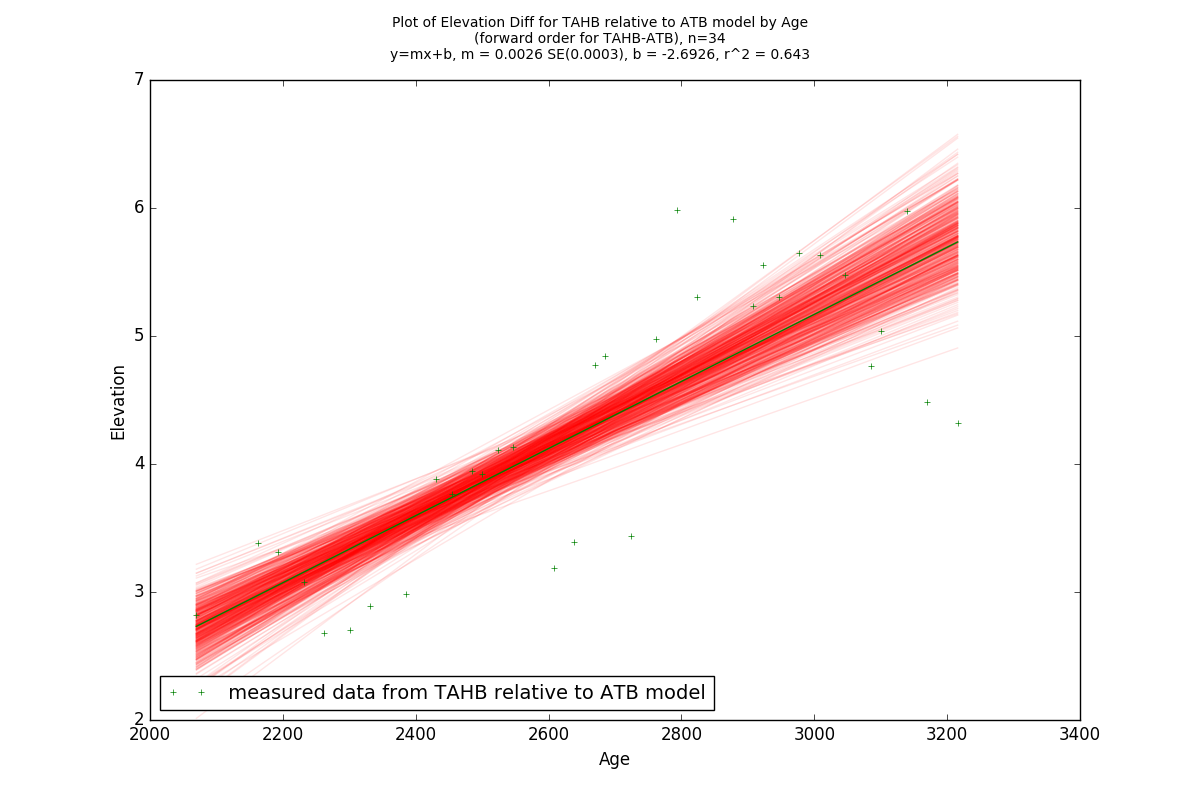
\includegraphics[width=1.7\linewidth, angle=270 ]{data/bothNonZero/withinSeventyFivePercent/gias/theGIA_TAHB_relative_to_ATB.png}
	\caption{Differences in elevation measured from the TAHB data to the ATB model. 95p Bootstrap of the main regression rendered in red around the estimator version of the regression (rendered as a solid green line).}
	\label{fig:gias_TAHBxATB}
\end{figure}
\newpage


\begin{figure}[H]
	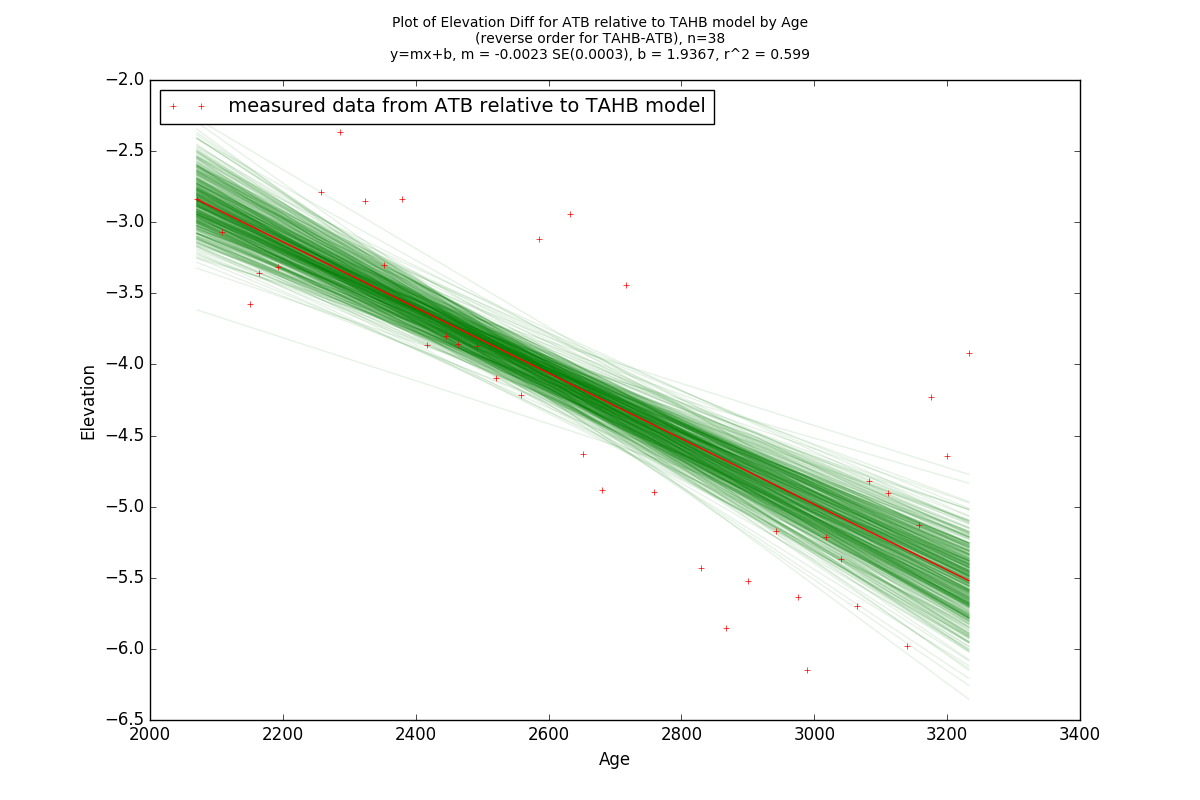
\includegraphics[width=1.7\linewidth, angle=270 ]{data/bothNonZero/withinSeventyFivePercent/gias/theGIA_ATB_relative_to_TAHB.png}
	\caption{Differences in elevation measured from the ATB data to the TAHB model. 95p Bootstrap of the main regression rendered in green around the estimator version of the regression (rendered as a solid red line).}
	\label{fig:gias_ATBxTAHB}
\end{figure}
\newpage




\subsubsection{GTB-BATB}

\begin{figure}[H]
	\makebox[\textwidth]{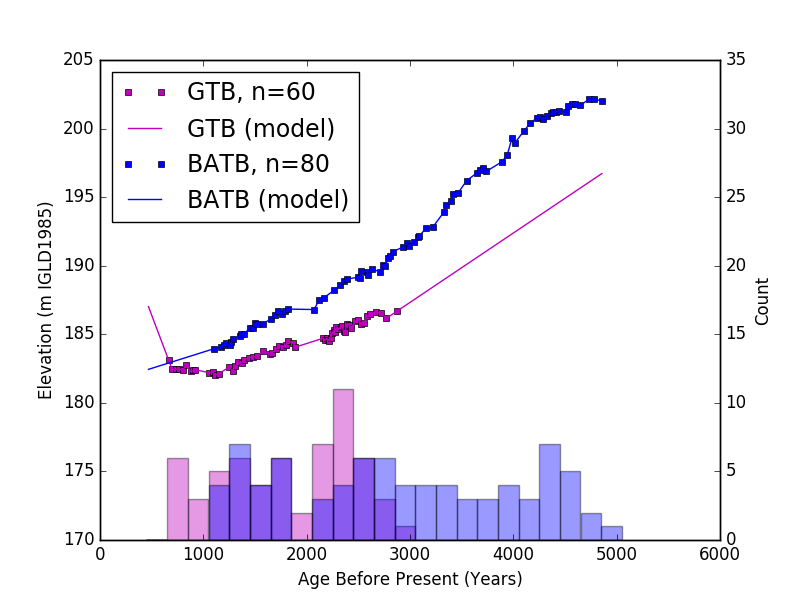
\includegraphics[width=0.72\paperwidth]{data/GTB-BATB_DataAndModel.png}}
	\caption{Measured and modelled elevation data plotted against age for sites GTB \& BATB. Data grouped into bins with widths of 200 years starting at 450 years before present. Bin Counts shown as a histogram at bottom of graph.}	
	\label{fig:data_GTBxBATB}
\end{figure}
The GTB BATB combination has data available for both datasets from 1050 to 3050 years before present with 
a gap in coverage from 1850 to 2050 years before present. The first case of the
75\% difference cutoff rule for bin inclusion has its first appearance here as
only the oldest shoreline available from GTB falls inside of the 2850-3050 years
before present window, causing the entire window to be
used if the only criteria was both dataset counts within that window being non-zero.
The 75\% cutoff prevents this window from being used in this case, as the counts
for the bin at 2850-3050 years before present differ by 120\% between GTB and BATB. This rule is useful in identifying
areas of the dataset where both sites have data available, but the density of
one of the datasets in that region is low enough to potentially cause inaccurate
predictions where modelled elevation extends a long distance between measured datapoints.
The regressions plotted in
Figures \ref{fig:gias_GTBxBATB} \& \ref{fig:gias_BATBxGTB} are listed in 
Figure \ref{fig:GTBxBATB_regression}. The $R^2$ values for both regressions
are well over 0.8, and the ranges for relative GIA listed under the "Slope C.I. (95p)" column
agree to within less than 1 cm/century,
producing one of the most well constrained values seen in this paper at 10.5-13.4 cm/century (a range of less than 3 cm/century). \\


\begin{figure}[H]
	\begin{flushleft}
	\csvautotabular[respect all]{data/GTB-BATB_regressionTable_bothNonZero_withinSeventyFivePercent.csv}
	\end{flushleft}
	\caption{GTB-BATB Regression output parameters}
	\label{fig:GTBxBATB_regression}
\end{figure}

\newpage

\begin{figure}[H]
	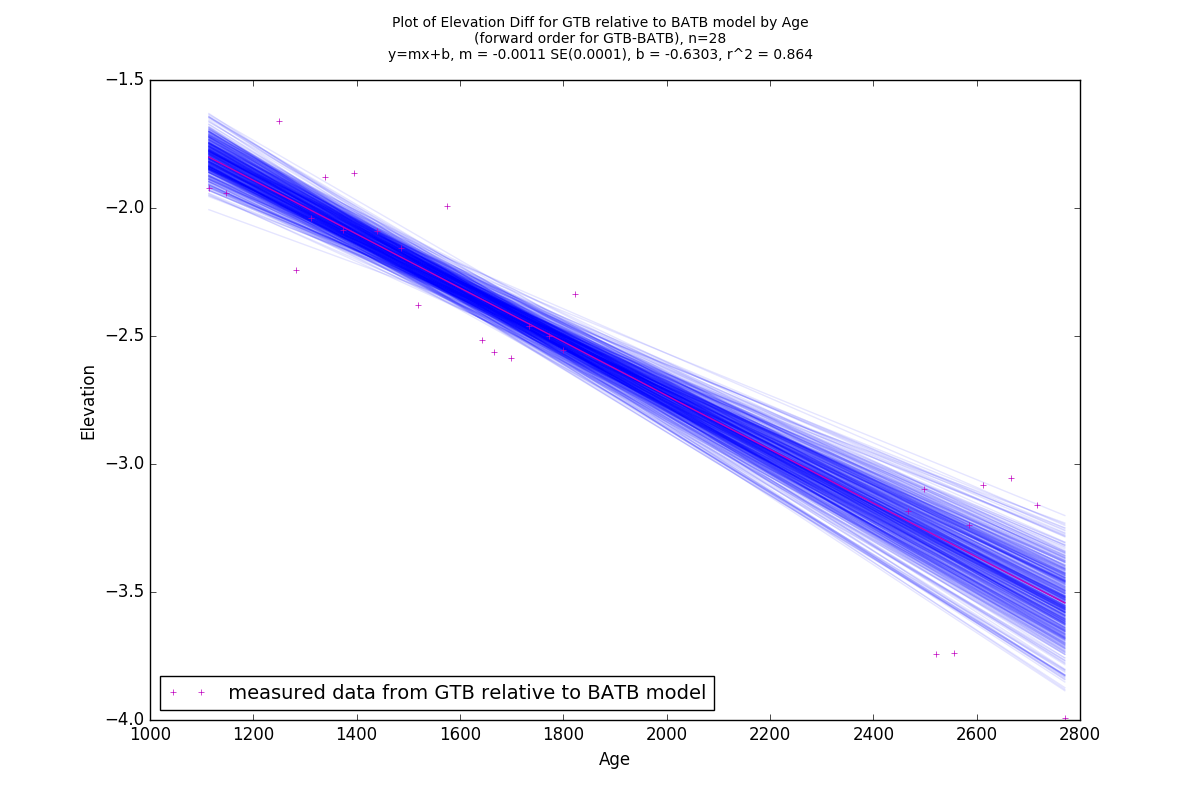
\includegraphics[width=1.7\linewidth, angle=270 ]{data/bothNonZero/withinSeventyFivePercent/gias/theGIA_GTB_relative_to_BATB.png}
	\caption{Differences in elevation measured from the GTB data to the BATB model. 95p Bootstrap of the main regression rendered in blue around the estimator version of the regression (rendered as a solid purple line).}
	\label{fig:gias_GTBxBATB}
\end{figure}
\newpage


\begin{figure}[H]
	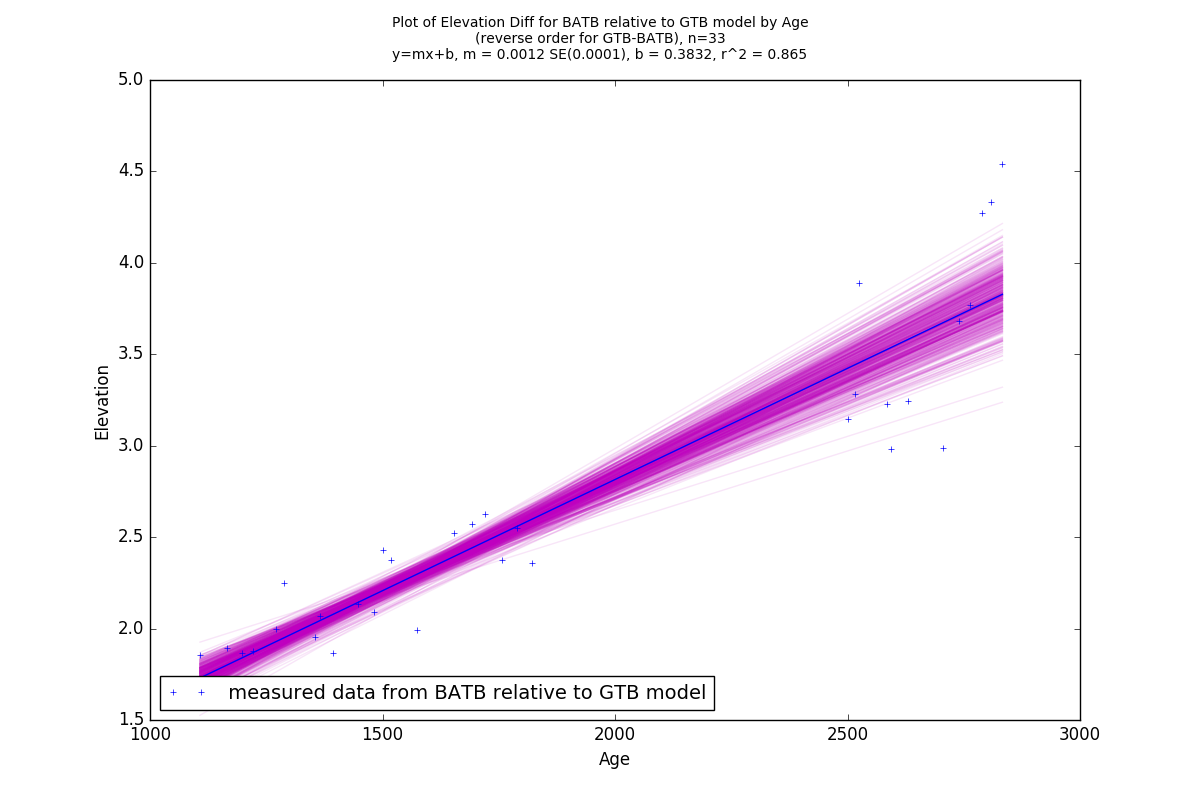
\includegraphics[width=1.7\linewidth, angle=270 ]{data/bothNonZero/withinSeventyFivePercent/gias/theGIA_BATB_relative_to_GTB.png}
	\caption{Differences in elevation measured from the BATB data to the GTB model. 95p Bootstrap of the main regression rendered in purple around the estimator version of the regression (rendered as a solid blue line).}
	\label{fig:gias_BATBxGTB}
\end{figure}
\newpage







\subsubsection{GTB-ATB}

\begin{figure}[H]
	\makebox[\textwidth]{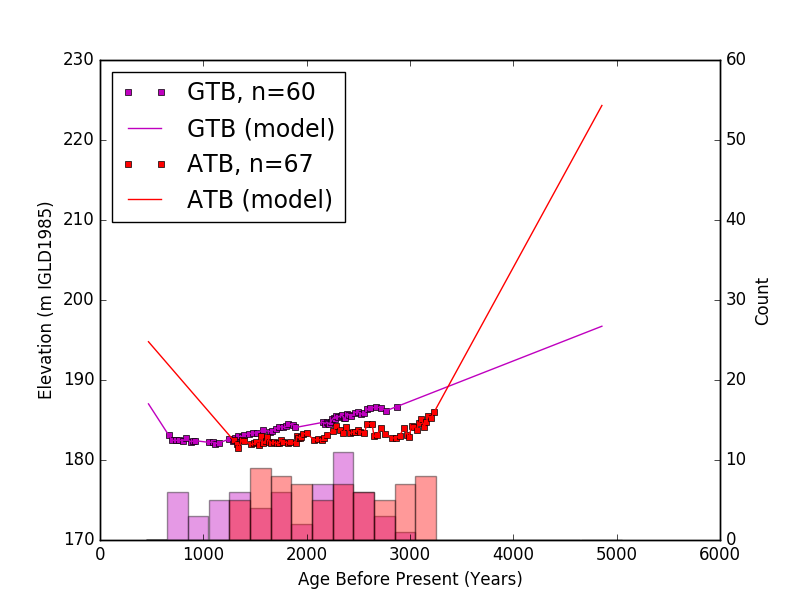
\includegraphics[width=0.72\paperwidth]{data/GTB-ATB_DataAndModel.png}}
	\caption{Measured and modelled elevation data plotted against age for sites GTB \& ATB. Data grouped into bins with widths of 200 years starting at 450 years before present. Bin Counts shown as a histogram at bottom of graph.}	
	\label{fig:data_GTBxATB}
\end{figure}

The GTB-ATB combination has
bins from 1250 to 3050 years before present containing data for both sites. Two of these bins
fail to qualify for use due to the site counts differing by more
than 75\%. These bins can be seen at 1850-2050, and 2850 to 3050 years before present. Looking
at Figure \ref{fig:data_GTBxATB}, it can be seen that both of these bins coincide with ranges of
time where GTB has sparse data, making the GTB models predictions unreliable in that bin.
The regressions plotted in Figures \ref{fig:gias_GTBxATB} \& \ref{fig:gias_ATBxGTB}, and
listed in Figure \ref{fig:GTBxATB_regression}. These regressions have weak correlations
(with $R^2$ values of 0.427 and 0.595 respectively), and only overlap in a small
range of 10.5-13.5 cm/century. Although this range appears very precise, the measurement
is likely inaccurate, as the comparisons do not agree very well between the forward
and reverse comparisons, the ranges of GIA produced from each regression only
overlapping for a small fraction of their respective ranges at the 95\% confidence
level.\\

\begin{figure}[H]
	\begin{flushleft}
	\csvautotabular[respect all]{data/GTB-ATB_regressionTable_bothNonZero_withinSeventyFivePercent.csv}
	\end{flushleft}
	\caption{GTB-ATB Regression output parameters}
	\label{fig:GTBxATB_regression}
\end{figure}

\newpage

\begin{figure}[H]
	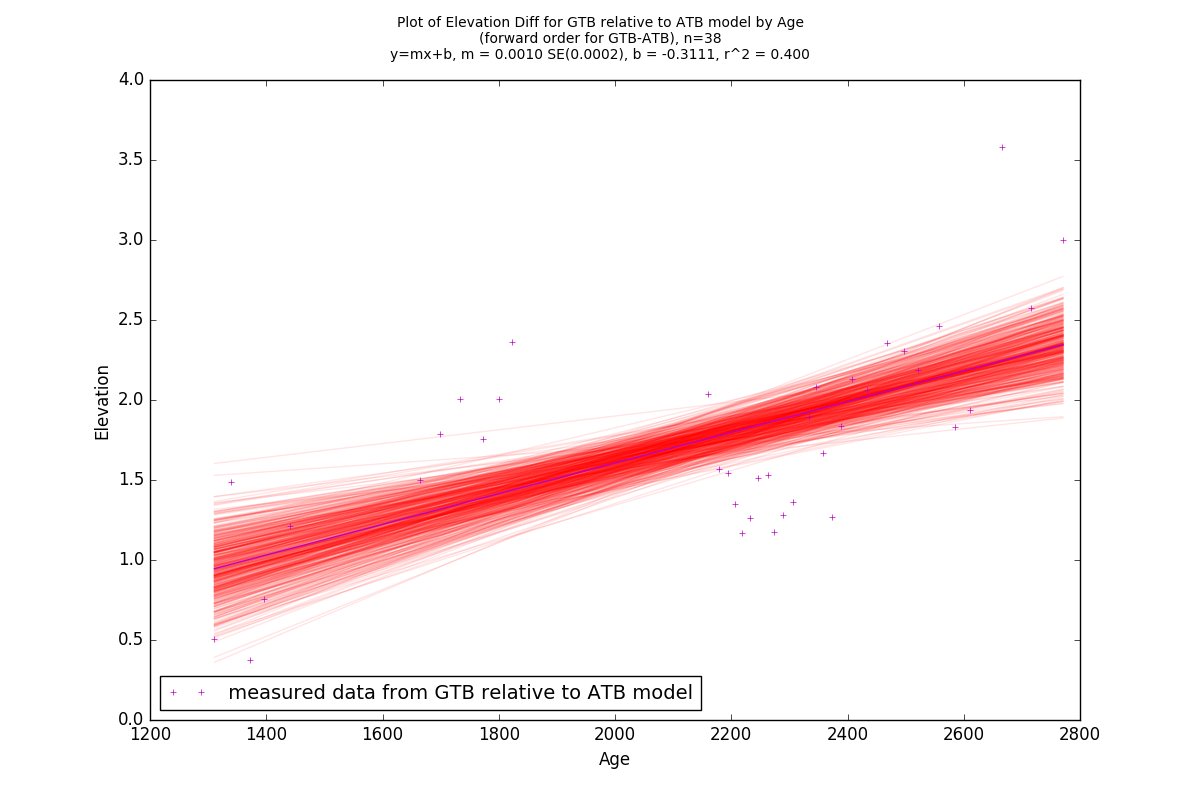
\includegraphics[width=1.7\linewidth, angle=270 ]{data/bothNonZero/withinSeventyFivePercent/gias/theGIA_GTB_relative_to_ATB.png}
	\caption{Differences in elevation measured from the GTB data to the ATB model. 95p Bootstrap of the main regression rendered in red around the estimator version of the regression (rendered as a solid purple line).}
	\label{fig:gias_GTBxATB}
\end{figure}
\newpage


\begin{figure}[H]
	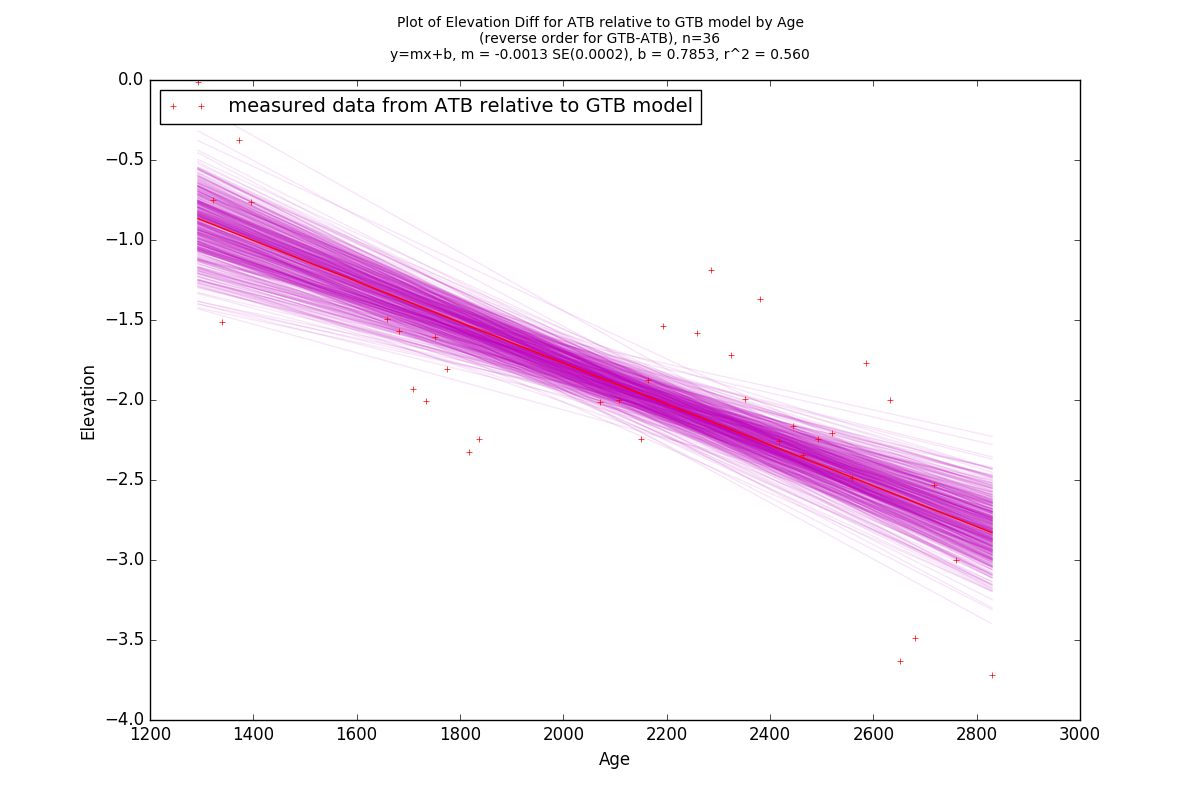
\includegraphics[width=1.7\linewidth, angle=270 ]{data/bothNonZero/withinSeventyFivePercent/gias/theGIA_ATB_relative_to_GTB.png}
	\caption{Differences in elevation measured from the ATB data to the GTB model. 95p Bootstrap of the main regression rendered in purple around the estimator version of the regression (rendered as a solid red line).}
	\label{fig:gias_ATBxGTB}
\end{figure}
\newpage








\subsubsection{GTB-TAHB}

\begin{figure}[H]
	\makebox[\textwidth]{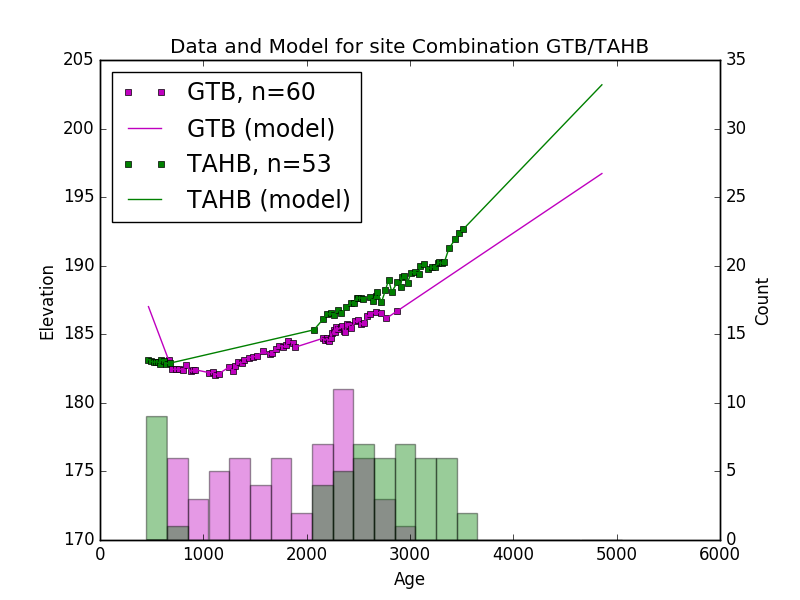
\includegraphics[width=0.72\paperwidth]{data/GTB-TAHB_DataAndModel.png}}
	\caption{Measured and modelled elevation data plotted against age for sites GTB \& TAHB. Data grouped into bins with widths of 200 years starting at 450 years before present. Bin Counts shown as a histogram at bottom of graph.}	
	\label{fig:data_GTBxTAHB}
\end{figure}
The combination of sites GTB and TAHB has data in bins from 450 to 3650 years before
present, of which only 2050 to 2850 years before present was used. Two
potential bins located at 650-850 and 2850-3050 years before present were not used due failing to
meet the 75\% rule, both would have produced comparisons between areas of
data in one dataset and a poorly constrained model in the other.

The combination of sites GTB and TAHB has by far the poorest regressions, listed
in \ref{fig:GTBxTAHB_regression}. This is likely due to the alignment of most
of both datasets only giving limited sample sizes of n=22 (Figure \ref{fig:gias_TAHBxGTB})
and n=27 (Figure \ref{fig:gias_GTBxTAHB}). 
This resulted in an estimate of GIA that ranges anywhere from -2.8-8.6 cm/century,
possibly implying that the vertical adjustment rates
between the TAHB and GTB sites may be zero, or at the least small in comparison to
other site comparisons. \\

\begin{figure}[H]
	\begin{flushleft}
	\csvautotabular[respect all]{data/GTB-TAHB_regressionTable_bothNonZero_withinSeventyFivePercent.csv}
	\end{flushleft}
	\caption{GTB-TAHB Regression output parameters}
	\label{fig:GTBxTAHB_regression}
\end{figure}

\newpage

\begin{figure}[H]
	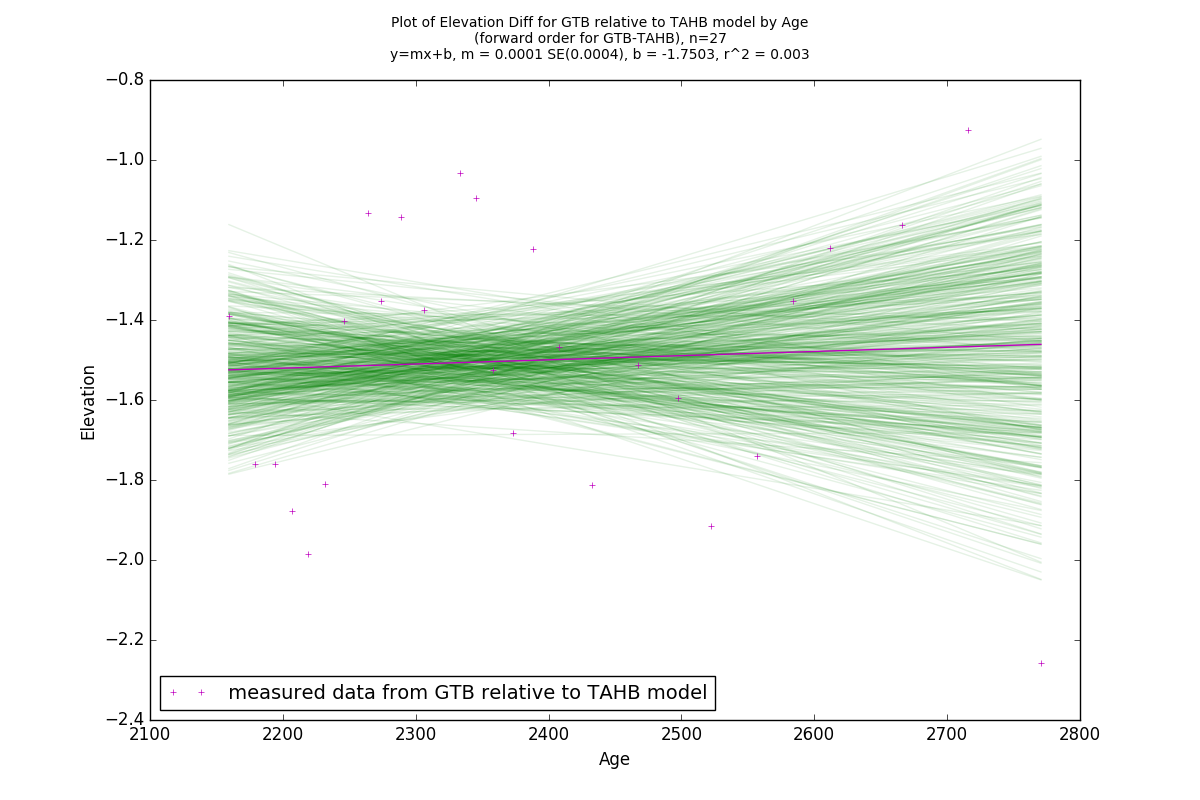
\includegraphics[width=1.7\linewidth, angle=270 ]{data/bothNonZero/withinSeventyFivePercent/gias/theGIA_GTB_relative_to_TAHB.png}
	\caption{Differences in elevation measured from the GTB data to the TAHB model. 95p Bootstrap of the main regression rendered in green around the estimator version of the regression (rendered as a solid purple line).}
	\label{fig:gias_GTBxTAHB}
\end{figure}
\newpage


\begin{figure}[H]
	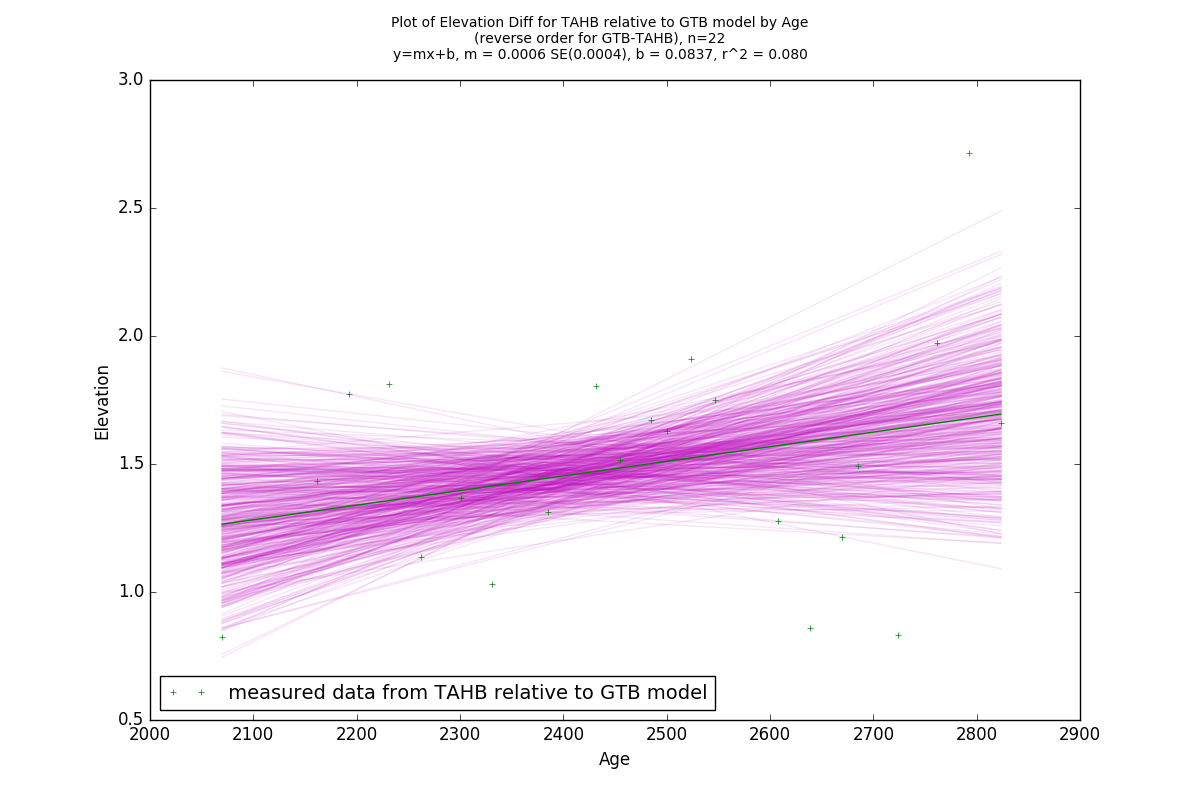
\includegraphics[width=1.7\linewidth, angle=270 ]{data/bothNonZero/withinSeventyFivePercent/gias/theGIA_TAHB_relative_to_GTB.png}
	\caption{Differences in elevation measured from the TAHB data to the GTB model. 95p Bootstrap of the main regression rendered in purple around the estimator version of the regression (rendered as a solid green line).}
	\label{fig:gias_TAHBxGTB}
\end{figure}
\newpage

\subsubsection{Complete Table of GIA Rate comparisons}

\begin{figure}[H]
	\makebox[\textwidth]{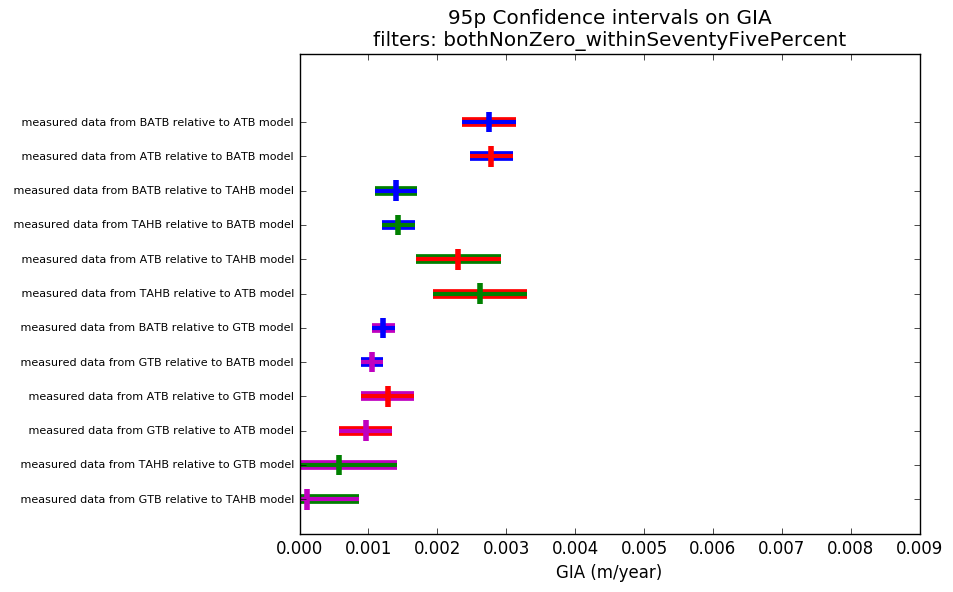
\includegraphics[width=0.6\paperwidth]{data/bothNonZero/withinSeventyFivePercent/gias/intervals.png}}
	\caption{95p Confidence intervals on absolute value of GIA rates obtained from 12 site comparisons across 4 sites.}
	\label{fig:intervalsGIA}
\end{figure}


\newpage




\subsubsection{Summary of calculated GIA values}

In Figure \ref{fig:myGIARates}, the values for relative GIA produced by this paper are
visualized by plotting the absolute value range of GIA rates between each site
as a line between sites on the map with the corresponding value next to it.

\begin{figure}[h]
	\makebox[\textwidth]{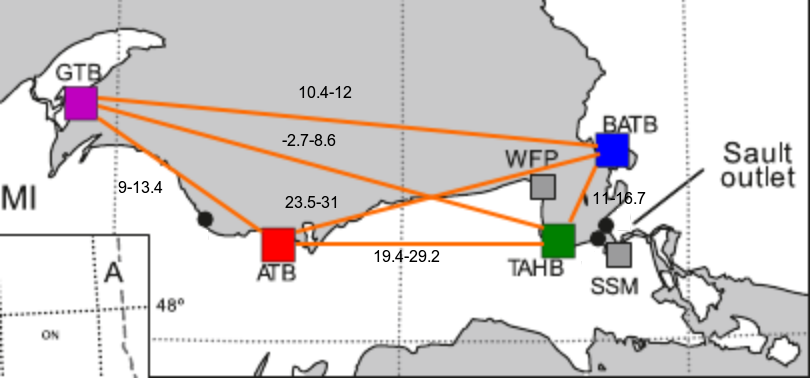
\includegraphics[width=0.72\paperwidth]{johnstonLaurentianMapWithMyGIARates.png}}
	\caption{Relative GIA Rates produced by this papers method, all values reported in cm/century}
	\label{fig:myGIARates}
\end{figure}
\newpage

The equivalent values for rates between sites as produced by Mainville \& Craymer
are inferred from subtracting the difference in contour between sites as shown in
Figure \ref{fig:craymerGIARatesBigPlot}, and are presented in Figure \ref{fig:craymerGIARates}.

\begin{figure}[h]
	\makebox[\textwidth]{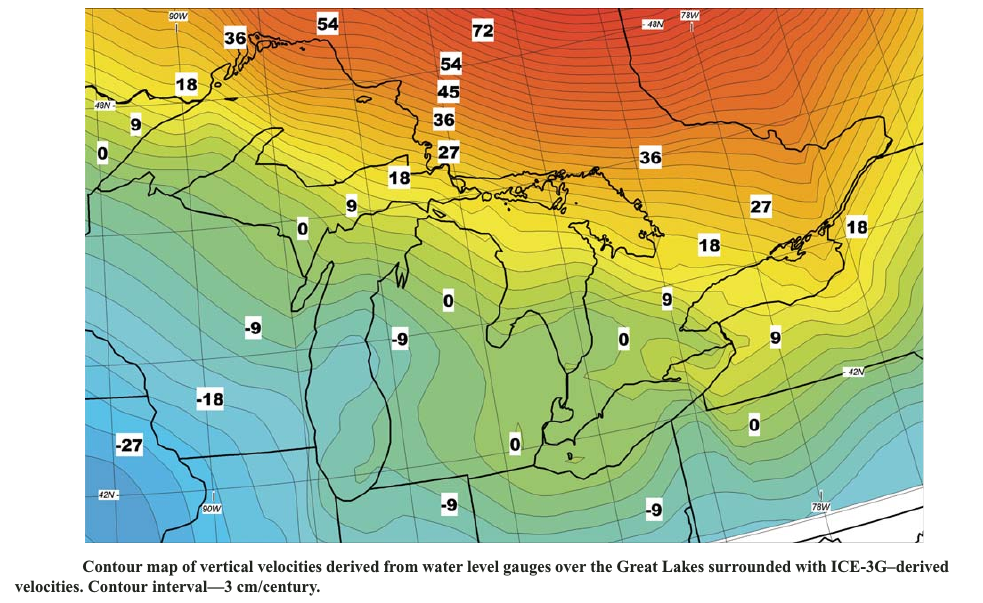
\includegraphics[width=0.72\paperwidth]{mainvilleGias.png}}
	\caption{Relative GIA Rates produced by Mainville \& Craymer, all values reported in cm/century (reproduced from Mainville \& Craymer, 2005)}
	\label{fig:craymerGIARatesBigPlot}
\end{figure}

\begin{figure}[h]
	\makebox[\textwidth]{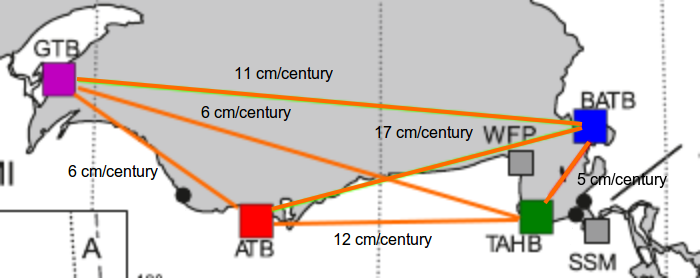
\includegraphics[width=0.72\paperwidth]{johnstonLaurentianMapWithCraymerGIARates.png}}
	\caption{Relative GIA Rates between this papers sites as reported by Mainville \& Craymer.}
	\label{fig:craymerGIARates}
\end{figure}
\newpage



Finally, the results of the analysis conducted in the previous section are summarized in
Figure \ref{fig:intervalsGIA}, which shows confidence intervals on absolute values of
rates of GIA for each and every site comparison calculated in Section 4. Each
pair of site comparisons is grouped in vertical order in order to show how each pair
of intervals overlaps, the range of GIA values in which they overlap is used as
the estimate of the absolute value GIA rate between the given pair of sites.

\newpage

\begin{figure}[H]
	\makebox[\textwidth]{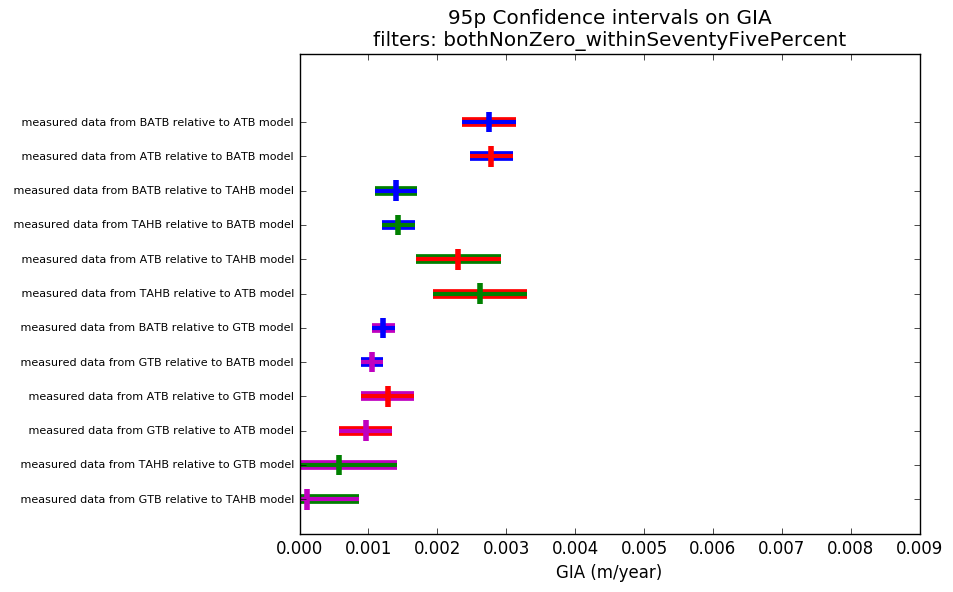
\includegraphics[width=0.6\paperwidth]{data/bothNonZero/withinSeventyFivePercent/gias/intervals.png}}
	\caption{Confidence intervals at the 95 \% confidence level for relative GIA rates obtained from 12 intra-site comparisons across 4 sites.}
	\label{fig:intervalsGIA}
\end{figure}

Comparing this papers results with those of Mainville \& Craymer, the value of
GIA reported by Mainville \& Craymer fell within the range reported by this paper
for 2 of the 6 pairs of sites (GTB \& TAHB and GTB \& BATB). For the remaining
four pairs of sites, the 95p confidence intervals on GIA calculated by this paper
tended to be larger than the equivalent values in Mainville \& Craymer, 
(namely ATB \& BATB, GTB \& ATB, and TAHB \& BATB) and sometimes much larger
(such as between ATB \& TAHB).

Given that the results of this paper are all on the same order of magnitude with
those reported by Mainville \& Craymer using data over a much shorter timescale,
this papers method can be inferred to be reasonably effective, but the
differences do need to be considered. These discrepancies may be an indication 
that the process of GIA in the LGL region behaved differently in the past than
in the more recent sample of time looked at by Mainville \& Craymer. One
particular area where significant
disagreement occurs is between sites ATB, BATB, and TAHB, especially in the much
larger values produced by this paper between ATB-BATB and ATB-TAHB. Given that both
of these site combinations are separated by an East-West line, this could imply
that the location of the center of the Laurentide Ice Sheet during the last glaciation being to the
north and west of Lake Superior had a stronger effect on the overall process of
rebound than the simple fact that areas to the north were more likely to be
depressed by the weight of ice sheets than areas further south. 

This interpretation should be taken with caution, given that the values produced
by this paper
may also be affected by differing quality of each intra-site measurement. Quality
of each GIA measurement is a subjective property, but it can be inferred that comparisons
that use as many data points as possible, which are evenly spread across as many 
200 year bins as possible, and have even quality between forward 
and reverse comparisons are more trustworthy than those that fail one or more of
those criteria. With that in mind, in the opinion of the Author of this paper,
the comparisons between GTB \& TAHB, GTB \& BATB, and TAHB \& ATB are of lesser
quality relative to the others. Coincidentally, two of these three comparisons
are those that agreed with Mainville \& Craymer, being lower in relative terms than
the rest of the comparisons. This could be interpreted to mean that the process of
GIA occurred at a higher rate over the longer periods of time studied by the
method of Johnston et al (2012) than it did over the shorter (and more recent)
span of time studied by that of Mainville \& Craymer (2005). Ultimately, this
conclusion is still an interpretation however, and the best method of determining
whether discrepancies between this papers method and previous ones would be to 
repeat the process with a dataset with better data coverage. One possible method
of accomplishing this would be further collection of data from sites already studied
in Johnston et al (2012), and by combining the data gathered from strandplains
closely spaced together around the lake basin.



\section{References}
Mainville, A., \& Craymer, M. R. (2005). Present-day tilting of the Great Lakes region based on water level gauges. Geological Society of America Bulletin, 117(7-8), 1070-1080.\\
Scott, T. W., Swift, D. J., Whittecar, G. R., \& Brook, G. A. (2010). Glacioisostatic influences on Virginia's late Pleistocene coastal plain deposits. Geomorphology, 116(1-2), 175-188.\\
Johnston, J. W., Argyilan, E. P., Thompson, T. A., Baedke, S. J., Lepper, K., Wilcox, D. A., \& Forman, S. L. (2012). A Sault-outlet-referenced mid-to late-Holocene paleohydrograph for Lake Superior constructed from strandplains of beach ridges. Canadian Journal of Earth Sciences, 49(11), 1263-1279.\\
Johnston, J. W., Thompson, T. A., \& Wilcox, D. A. (2014). Palaeohydrographic reconstructions from strandplains of beach ridges in the Laurentian Great Lakes. Geological Society, London, Special Publications, 388(1), 213-228.\\

\newpage

\section{Appendix}
\foreach \python in  {giaModel.py, giaUtils.py , rawhide/bootstrapper.py, rawData.py, dataModel.py, linearInterpolationModel.py}
{
	\subsection{Source code for \textsf{\python}}
	\lstinputlisting[language=python]{./data/\python}
	\newpage
	
}



\end{document}
